
%(BEGIN_QUESTION)
% Copyright 2012, Tony R. Kuphaldt, released under the Creative Commons Attribution License (v 1.0)
% This means you may do almost anything with this work of mine, so long as you give me proper credit

Explain how each of the following pressure instruments works, identifying whether each one uses the principle of {\it motion-balance} or the principle of {\it force-balance}.  Please note that a series of angled lines projecting from a vertical or horizontal line represents a point of anchoring, where that horizontal or vertical surface is stationary:

\vskip 10pt

\noindent
{\bf Example 1:}

$$\includegraphics[width=15.5cm]{i00208x01.eps}$$

\vskip 10pt

\filbreak

\noindent
{\bf Example 2:}

$$\includegraphics[width=15.5cm]{i00208x02.eps}$$

\vskip 10pt

\filbreak

\noindent
{\bf Example 3:}

$$\includegraphics[width=15.5cm]{i00208x03.eps}$$

\vskip 10pt

\filbreak

\noindent
{\bf Example 4:}

$$\includegraphics[width=15.5cm]{i00208x04.eps}$$

\vskip 10pt

\filbreak

\noindent
{\bf Example 5:}

$$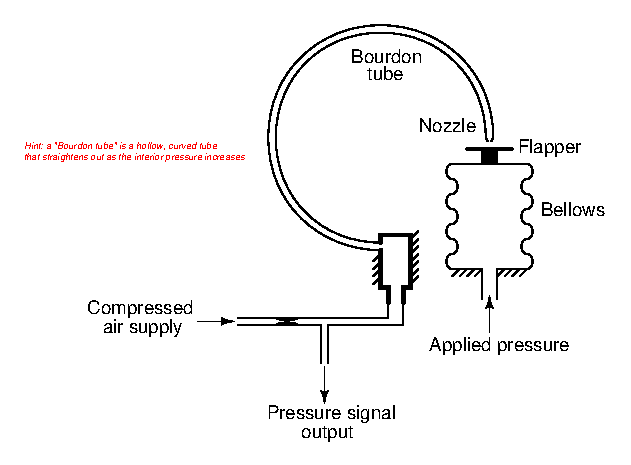
\includegraphics[width=15.5cm]{i00208x05.eps}$$

\vskip 10pt

\filbreak

\noindent
{\bf Example 6:}

$$\includegraphics[width=15.5cm]{i00208x06.eps}$$

\vskip 10pt

\filbreak

\noindent
{\bf Example 7:}

$$\includegraphics[width=15.5cm]{i00208x07.eps}$$

\vskip 10pt

\filbreak

\noindent
{\bf Example 8:}

$$\includegraphics[width=15.5cm]{i00208x08.eps}$$

\vskip 10pt

\filbreak

\noindent
{\bf Example 9:}

$$\includegraphics[width=15.5cm]{i00208x09.eps}$$





\vskip 20pt \vbox{\hrule \hbox{\strut \vrule{} {\bf Suggestions for Socratic discussion} \vrule} \hrule}

\begin{itemize}
\item{} The distinction between force-balance and motion-balance is one that tends to confuse students.  A common tactical error students make is to attempt to memorize distinguishing characteristics in order to identify what type of balancing a particular mechanism employs.  A better approach is to {\it think through} the operation of such pneumatic mechanisms using ``thought experiments'' to identify which balance principle they employ.  Why do you think it is bad to go with the memorization approach instead of the ``thought experiment'' approach?
\item{} What difference does it make to us (as technicians) to know whether a mechanism is force- or motion-balance?  In other words, who cares???
\item{} Identify changes that could be made to each mechanism in order to alter its {\it zero}.
\item{} Identify changes that could be made to each mechanism in order to alter its {\it span}.
\item{} An interesting ``thought experiment'' to run is to modify some aspect of the mechanism (e.g. stiffer spring, greater supply air pressure, relocating the orifice) and re-analyze that mechanism to see what effect(s) that change will have on its operation.
\end{itemize}

\underbar{file i00208}
%(END_QUESTION)





%(BEGIN_ANSWER)

\begin{itemize}
\item{}(1) Force-balance 
\item{}(2) Motion-balance 
\item{}(3) Force-balance 
\item{}(4) Force-balance 
\item{}(5) Motion-balance 
\item{}(6) Motion-balance 
\item{}(7) Force-balance 
\item{}(8) Motion-balance 
\item{}(9) Force-balance 
\end{itemize}

The general principle to keep in mind here is that motion-balance instruments generate a {\it motion} to counteract an input motion in order to maintain a constant detector (flapper/nozzle) gap, while force-balance instruments generate a {\it force} to counteract an input force in order to maintain a constant detector (flapper/nozzle) gap.

\vskip 10pt

Example number 9 is tricky, because one might argue it is {\it motion-balance} by virtue of the lower bellows' stretching motion as output pressure increases.  However, the fact that the two bellows' forces oppose each other to ensure the flapper remains {\it stationary} in order to hold a constant flapper/nozzle gap is a defining characteristic of any force-balance mechanism.  Also, the degree of spring stiffness has no effect whatsoever on the gain of this mechanism, which it would if it were motion-balance (i.e. if the amount of motion generated per unit increase in output pressure were related at all to the amount of input pressure increase).  The two bellows' {\it forces} will cancel each other to achieve equilibrium regardless of how much or how little the spring must compress in the process of achieving that balance.  If this were a true motion-balance mechanism, weakening the spring (making it less stiff) would result in a decrease of output pressure because less pressure would be required to move as far as before.  Here, a weakened spring would indeed result in the lower bellows expanding a greater distance than before to balance the same amount of input pressure, but this would actually be the same output pressure as before, meaning the change in required motion has no effect on the gain.

%(END_ANSWER)





%(BEGIN_NOTES)

The flexible tube in example \#7 is gratuitous: I put it there just to fool students who try to associate motion-balance instruments with the presence of flexible tubes.  The flexible tube in example \#9 is actually necessary, but it doesn't change the fact that \#9 is still a force-balance mechanism.

%INDEX% Measurement, pressure: motion- versus force-balance

%(END_NOTES)


